\begin{frame}{Tor}
    \begin{itemize}
    \item Tor --- ``onion routing''
    \item suppose connecting from A to B and A to C
    \item goal: connection is anonymous
    \item method: proxy through several `onion routers'
    \vspace{.5cm}
    \item attacker should only know:
        \begin{itemize}
        \item A is sending to someone via Tor
        \item B is receiving from someone via Tor
        \item C is receiving from someone via Tor
        \end{itemize}
    \item not be able to tie A and B or A and C or B and C together otherwise
    \end{itemize}
\end{frame}

\begin{frame}{Tor threat model}
    \begin{itemize}
    \item (from Digledine, Mathewson, Syverson, ``Tor: A Second-Generation Onion Router'')
    \item an advserary ``who can observe some fraction of network traffic; who can generate, modify,
        delete, or delay traffic; who can operate onion routers of their own; and who can compromise some
        fraction of onion routers''
    \end{itemize}
\end{frame}

\begin{frame}{Tor circuit idea (1)}
    \begin{itemize}
    \item $E_X(Y)$ = Y encrypted to X
    \item to create `circuit': A $\leftrightarrow$ OR1 $\leftrightarrow$ OR2 $\leftrightarrow$ B
        \begin{itemize}
        \item OR = onion router
        \item can choose different number of ORs if desired
        \end{itemize}
    \item A sends OR1 via TLS: \\
        ``please setup circuit to OR2: '' + $E_{OR2}$(``please setup circuit to B'')
    \item OR1 sends A's encrypted data to OR2 with OR1's circuit ID
    \item OR2 sends back responses via OR1 + OR1's circuit iD
    \item OR1 uses circuit ID to send back to A
    \end{itemize}
\end{frame}

\begin{frame}{Tor circuit idea (2)}
    \begin{itemize}
    \item A $\leftrightarrow$ OR1 $\leftrightarrow$ OR2 $\leftrightarrow$ B
    \vspace{.5cm}
    \item OR1 doesn't know who A is sending to
    \item OR2 doesn't know who is sending to B
    \item fine if OR1, OR2 independently operated
        \begin{itemize}
        \item in practice: probably add additional OR to circuit
        \item otherwise, require large portion of ORs to be independent
        \end{itemize}
    \end{itemize}
\end{frame}

\begin{frame}{Tor circuit}
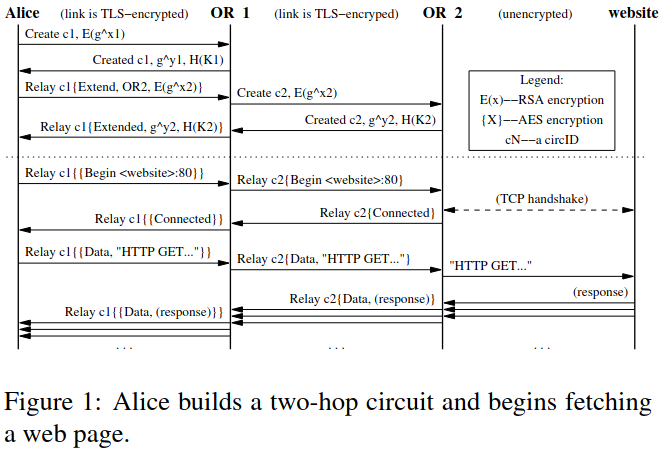
\includegraphics[heigth=0.9\textheight]{../encap/tor-fig1}}
\end{frame}

\begin{frame}{traffic analysis problem}
    \begin{itemize}
    \item problem 1: if I see A send 1000 bytes, then receive 1749 bytes, and\ldots
    \item at about the same time I see B receive 1000 bytes, then send 1749 bytes
    \item \ldots would be a big tell
    \vspace{.5cm}
    \item worse: B or OR 1 or OR 3 can deliberately generate patterns of traffic to help ID A
    \end{itemize}
\end{frame}

\begin{frame}{mitigations for traffic analysis?}
    \begin{itemize}
    \item general idea: add data or delay to make everything `the same'
    \item add padding to traffic sent on `circuit'
        \begin{itemize}
        \item 512-byte cells only (can't see exact sizes in bytes)
        \item additional padding cells added, too
        \end{itemize}
    \item ``cover traffic'' sent periodically between A and OR1
        \begin{itemize}
        \item 1.5 s to 9.5 s in each direction if no traffic
        \item idea: hard for attacker to tell when user active
        \end{itemize}
    \item but real-time nature limits possible mitigations
        \begin{itemize}
        \item similar idea for email avoids with random delays
        \item \ldots but can't really browse the web that way
        \end{itemize}
    \end{itemize}
\end{frame}

\begin{frame}{application-layer tells}
    \begin{itemize}
    \item browser reveals a lot of information:
        \begin{itemize}
        \item browser, OS version
        \item screen size
        \item fonts available
        \item timezone
        \item \ldots
        \end{itemize}
    \item problematic for anonymity
        \begin{itemize}
        \item helps B limit possible other ends very seriously
        \end{itemize}
    \vspace{.5cm}
    \item Tor browser (modified Firefox, essentially) mitigation: \\
        limited set of screen sizes, OS versions, fonts, etc. allowed
    \end{itemize}
\end{frame}

\begin{frame}{other Tor browser paranoia}
    \begin{itemize}
    \item scripts disabled by default
        \begin{itemize}
        \item seriously limits `ordinary' browser security vulnerabilities
        \end{itemize}
    \item cookies, caches cleared when browser closed
    \item HTTPS-only by default
        \begin{itemize}
        \item really dangerous otherwise since we don't trust last onion router
        \end{itemize}
    \end{itemize}
\end{frame}
